\section{Model from template protocol}
\label{app:modelFromTemplate}%a110
Protocol designed to obtain a structure model for a target sequence in \scipion. Target structure is predicted by sequence homology using \modeller \citep{sali1993} web service in \chimera.\\
WARNING: Working with \modeller requires a license key, which can be requested free of charge for academic users. Try to have this license key before starting the protocol execution.\\ 

   
 \begin{itemize}
  \item \scipion menu:\\
  \ttt{Protocols SPA -> Model building} (\ffigure{fig:app_protocol_seqHomology_1} (A))\\
  
  \item Protocol form parameters (\ffigure{fig:app_protocol_seqHomology_1} (B)):\\
  
  \begin{figure}[H]
    \centering 
    \captionsetup{width=.7\linewidth} 
    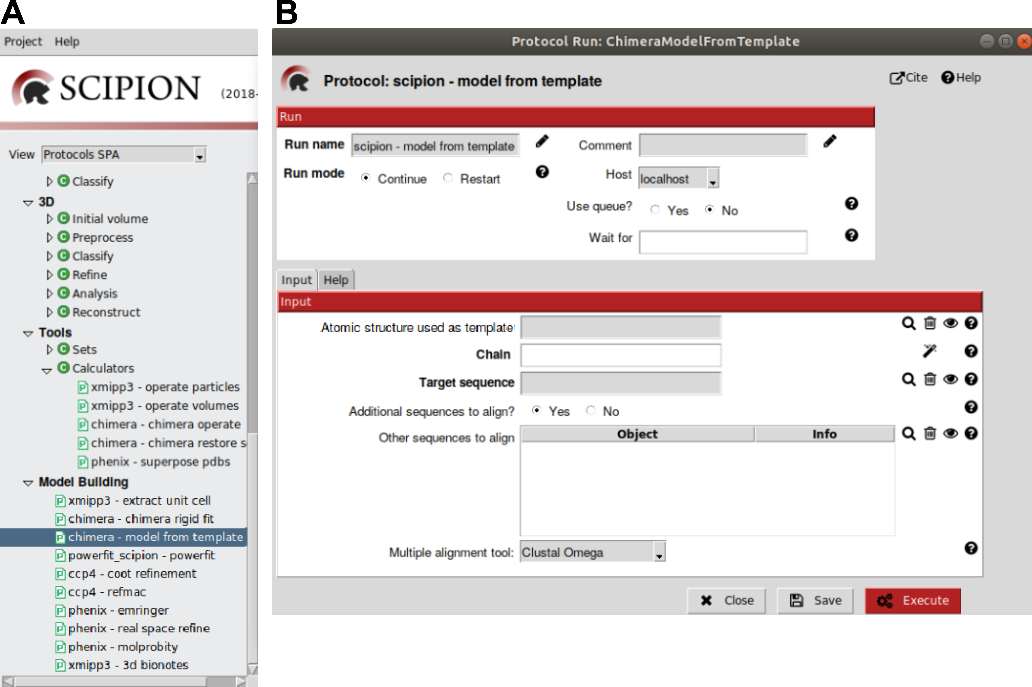
\includegraphics[width=0.90\textwidth]{Images_appendix/Fig111.pdf}
    \caption{Protocol \scommand{model from template}. A: Protocol location in \scipion menu. B: Protocol form.}
    \label{fig:app_protocol_seqHomology_1}
   \end{figure}
  
  \begin{itemize}
   \item \ttt{Input} section\\
  

  \begin{itemize}
   \item \ttt{Atomic structure used as template}: Atomic structure previously downloaded in \scipion. This structure was selected by sequence homology, i.e. by looking for the structurally characterized sequence more similar (with higher identity) to the target sequence.\\
   \item \ttt{Chain}: Specific monomer of the macromolecule that has to be used as structure template of the target sequence. Use the wizard at the right side of \ttt{Chain} parameter to select that chain.\\
   \item \ttt{Target sequence}: Sequence previously downloaded in \scipion. This sequence has to be modeled following the structure skeleton of the selected template.\\
   \item \ttt{Additional sequences to align?}: $Modeller$ provides structural models of the target sequence based on a sequence alignment, in which at least sequences of template and target have to be included. Set to "No" this form parameter if no more sequences are going to be included in the alignment. Nevertheless, set the parameter to "Yes" if you want to perform a multiple sequence alignment. Additional sequences, others than template and target sequences, are required to accomplish this multiple alignment. That's why a new form parameter appear with the option "Yes":\\
    \begin{itemize}
	 \item \ttt{Other sequences to align}: Box to complete with the additional sequences used to perform the multiple sequence alignment. All of them were previously downloaded in \scipion.\\
	\end{itemize}
   \item \ttt{Multiple alignment tool}: Multiple option box to select an alignment program. Three possible options are given for pairwise alignments (\ttt{Bio.pairwise2, Clustal Omega, MUSCLE}) whereas only the two last ones are allowed for multiple sequence alignments.\\
   \end{itemize}
   
  \item \ttt{Help} section\\
  
  Follow this section steps to run $Modeller$ via web service in \chimera and to select and save one of the retrieved models in \scipion framework.\\
  
  \end{itemize}
  \item Protocol execution:\\
  
  Adding specific template-target label is recommended in \ttt{Run name} section, at the form top. To add the label, open the protocol form, press the pencil symbol at the right side of \ttt{Run name} box, complete the label in the new opened window, press OK, and finally, close the protocol. This label will be shown in the output summary content (see below). If you want to run again this protocol, do not forget to set to \ttt{Restart} the \ttt{Run mode}.\\
  Press the \ttt{Execute} red button at the form bottom.\\
  
  Several \chimera windows will be opened after executing the protocol. The two more relevant are \chimera graphics window and the multiple alignment window. In both windows the template chain is shown highlighted (see an example of these windows in \ffigure{fig:chimera_alignment}). Main steps to follow ahead are:\\
  \begin{itemize}
   \item Edit the alignment if needed. Sequences can be renamed, added, deleted, etc.. in the upper menu of the multiple sequence alignment window (\ttt{Edit -> }).\\
   \item Send this alignment to $Modeller$ by selecting \ttt{Structure -> Modeller (homology ...)} in the upper menu of the multiple sequence alignment window.\\ 
   \item Complete the new window opened for \ttt{Comparative Modeling with Modeller} (\ffigure{fig:app_protocol_seqHomology_2} (A)) with \iii{target} sequence (1), \iii{template} (2), Modeller license key (3) and Advanced options like the number of models retrieved by \modeller (4), as well as $model$ inclusion of heteroatoms (5) or water molecules (6). By pressing \ttt{Apply} or \ttt{OK} (5) the computation starts without hiding and hiding this panel window, respectively. The status of the job can be checked in the lower left corner of \chimera graphics window.\\
   \item After a while a new panel window will show retrieved models of the target sequence (\ffigure{fig:app_protocol_seqHomology_2} (B)). Two statistics assess these models: \ttt{GA341}, statistical potentials derived-score, (1) and \ttt{zDOPE}, normalized Discrete Optimized Protein Energy, atomic distance depending-score (2). Reliable models show GA341 values higher than 0.7, and negative zDOPE values correspond to better models. One of the retrieved models has to be selected. Selected model and the rest of models can be checked in \chimera \ttt{Favorites -> Model Panel}.\\
   \item Save the retrieved model selected according to the model number (\ttt{\#n}) shown in \chimera \ttt{Favorites -> Model Panel} by writing in \chimera \ttt{Favorites -> Command Line}:\\\ttt{scipionwrite model \#n}.\\
  \end{itemize}
  
 
  \begin{figure}[H]
  \centering 
  \captionsetup{width=.7\linewidth} 
  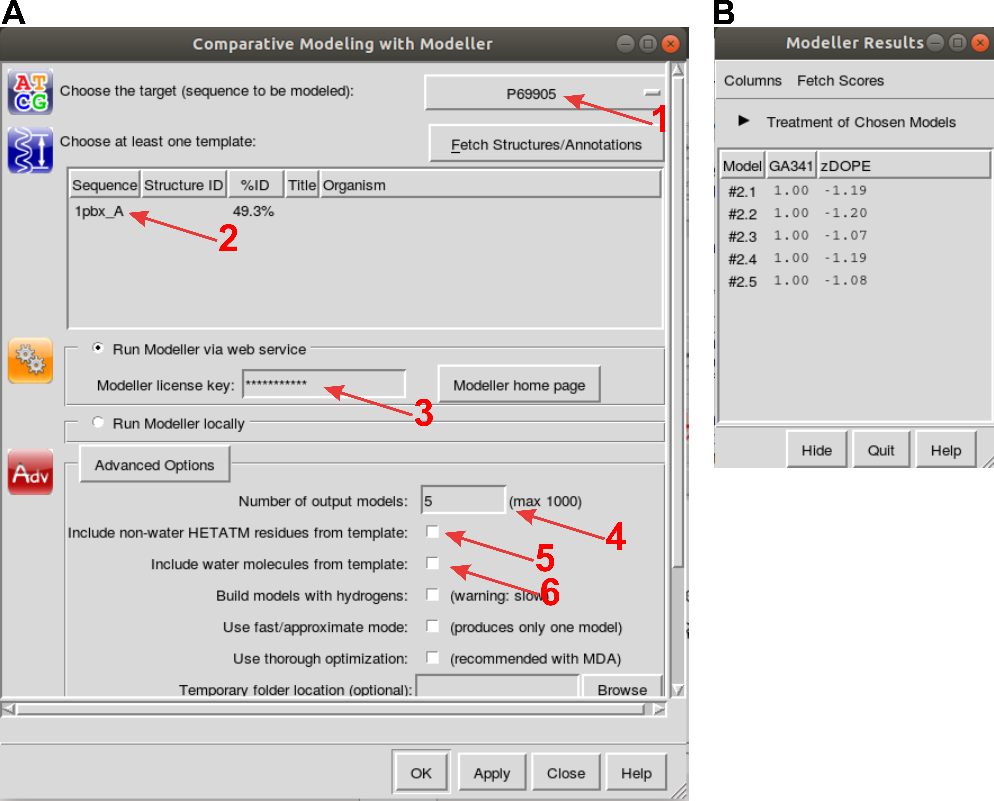
\includegraphics[width=0.80\textwidth]{Images_appendix/Fig112.pdf}
  \caption{(A) Form to access to homology modeling with \modeller. (B) Panel window of \modeller retrieved models.}
  \label{fig:app_protocol_seqHomology_2}
  \end{figure}

  \item Visualization of protocol results:\\
  
  After executing the protocol, press \ttt{Analyze Results} and \chimera graphics window will be opened by default. 
  Atomic structures are referred to the origin of coordinates in \chimera . To show the relative position of the atomic structure, the three coordinate axes are represented; X axis (red), Y axis (yellow), and Z axis (blue) (\ffigure{fig:app_protocol_volume_3}). Coordinate axes and imported atomic structure are model numbers \ttt{\#0} and \ttt{\#1}, respectively, in \chimera \ttt{Model Panel}.\\
   
   \item Summary content:\\
    \begin{itemize}
     \item Protocol output (below \scipion framework):\\ \ttt{scipion - model from template -> ouputPdb\_01}; \ttt{Pdbfile (pseudoatoms=True/ False, volume=True/ False)}.\\Pseudoatoms is set to \ttt{True} when the structure is made of pseudoatoms instead of atoms. Volume is set to \ttt{True} when an electron density map is associated to the atomic structure.\\
     \item \ttt{SUMMARY} box:\\Produced files:\\chimeraOut0001.pdb\\we have some result\\
    \end{itemize}
  
  \end{itemize}
